\documentclass[conference]{IEEEtran}
\IEEEoverridecommandlockouts
% The preceding line is only needed to identify funding in the first footnote. If that is unneeded, please comment it out.
\usepackage{caption}
\usepackage{biblatex}
\usepackage{amsmath,amssymb,amsfonts}
\usepackage{algorithmic}
\usepackage{graphicx}
\usepackage{textcomp}
\usepackage{xcolor}
\usepackage{listings}
\usepackage{url}
\usepackage{pgfplots}
\usepackage{newtxtext,newtxmath}
\usepackage{hyperref}

\pgfplotsset{compat=1.18}

\definecolor{mGreen}{rgb}{0,0.6,0}
\definecolor{mGray}{rgb}{0.5,0.5,0.5}
\definecolor{mPurple}{rgb}{0.58,0,0.82}
\definecolor{backgroundColour}{rgb}{0.95,0.95,0.92}

\def\BibTeX{{\rm B\kern-.05em{\sc i\kern-.025em b}\kern-.08em
    T\kern-.1667em\lower.7ex\hbox{E}\kern-.125emX}}
    \bibliography{ref}
\addbibresource{ref.bib}

\lstdefinestyle{CStyle}{
    backgroundcolor=\color{backgroundColour},   
    commentstyle=\color{mGreen},
    keywordstyle=\color{magenta},
    numberstyle=\tiny\color{mGray},
    stringstyle=\color{mPurple},
    basicstyle=\footnotesize,
    breakatwhitespace=false,         
    breaklines=true,                 
    captionpos=b,                    
    keepspaces=true,                 
    numbers=left,                    
    numbersep=8pt,                  
    showspaces=false,                
    showstringspaces=false,
    showtabs=false,                  
    tabsize=2,
    language=C
}

\begin{document}
\title{Parallelizing Matrix Transposition 2024-2025}

\author{
    \IEEEauthorblockN{Matteo Gottardelli 237749}
    \IEEEauthorblockA{\textit{Computer, Communication, and Electronics Engineering}\\
    University of Trento, Italy\\
    Email: matteo.gottardelli@studenti.unitn.it}
}

\maketitle
\begin{abstract}
This study explores methods for transposing an N$\times$N matrix, focusing on parallelization of a sequential code involving a symmetry check followed by transposition if needed.
Parallelization was achieved using both implicit parallelism (block-based and recursive strategies) and OpenMP (OMP).
Performance was analyzed by comparing execution times, speedups, and efficiency for different methods, matrix sizes, and thread counts.
Simulations were conducted on the University of Trento’s cluster, with nodes having 64 CPUs, 64 OMP threads, and 1 GB of memory.
Results show that for implicit parallelism, the block-based approach slightly outperformed the recursive method, especially for larger matrices.
The OMP implementation exhibited overhead for small matrices (N$\leq 2^6$), but speedup improved significantly for larger sizes (N$\geq 2^{10}$), with efficiency peaking at 16 threads before bottlenecks appeared.
\end{abstract}
\section{Introduction}
Matrix transposition is a fundamental operation in linear algebra. It involves swapping the first row of a matrix with its first column, and this procedure is repeated for each subsequent row.
The goal of this project is to transpose matrices of varying sizes using different numbers of threads and parallel algorithms. This application is useful in fields like robotics, where the transpose of an orthogonal matrix is equal to its inverse , so having a valuable algorithm may help to solve operations such as inverse kinematics.
For small-sized problems, parallelization may not significantly impact performance. However, for simulations involving large, optimizing computational time becomes crucial. This project addresses the problem by simplifying the hypothesis with matrices having dimensions that are powers of two, with equal numbers of rows and columns (square matrices).
When working with small matrices, operations can be performed quickly, often without requiring parallelism, as the overhead might outweigh the benefits. However, as matrix size increases, computation time grows exponentially. This will be evident in the breakdown of sequential code execution. Thus, implementing strategies to reduce computational time is essential.
The objective of this project is to analyze the average execution times recorded for various simulations and compare them with sequential code, considering specific requirements (matrix size, test mode, and number of threads). These implied strategies from both implicit and explicit (OMP) parallelism’s algorithms. By comparing speedups and efficiencies, the project aims to identify the most efficient parallelization method and investigate potential bottlenecks associated with particular matrix sizes or thread counts.
The simulations were conducted on the University of Trento's cluster, featuring an x86-64 architecture node capable of supporting at least 64 CPUs, 64 OMP threads, and a minimum of 1 GB of memory. Detailed information on reproducing the results is available on the project's GitHub page, linked in the bibliography. 
\section{State-of-the-art}
To explore existing solutions, I’ve investigated the article \cite{cache_efficiency}. It proposes a series of transposition algorithms aimed at reducing I/O complexity, and I will cite the two most efficient ones.
The first algorithm (Algorithm 2) is a block-based one, which aims to divide the matrix N$\times$ N into B$\times$B submatrices, leveraging spatial locality to minimize memory accesses.
It assumes that N is a multiple of B. This algorithm operates on each row's elements, but when accessing the next row, the value has to be searched in memory, because we need to consider that they are distant N-B elements.
Computationally, each iteration will involve one read and one write, leading to $2\cdot \frac{N^2}{B^2}\cdot B^2=2N^2$ computations. This block transpose algorithm doesn't depend on B, the subblock size, but it is affected by the execution time because B must be chosen appropriately to accommodate the memory size. If B is too large ($B^2\geq cache\,memory$), the algorithm may not be efficient anymore.
The other algorithm uses a nonlinear layout function called Morton ordering \cite{morton_ordering}, which aims to map a 2D matrix into a 1D mapping, ideal for spatial locality, because it minimizes cache misses. The authors use a recursive approach, dividing the original matrix into four submatrices until reaching a small one, like B in the first algorithm. To satisfy the conditions of this algorithm, the following must hold: $\frac{m}{t_R}=\frac{n}{t_c}=2^d$, where mm and nn are the number of rows and columns, and $t_R$, $t_C$ are the sizes of the smaller submatrices.
The limitation in this algorithm is that it requires mapping into 1D to preserve locality, but with high numbers it isn't uniform. Computationally, each submatrix has $2B^2$ and it creates other 4 matrices with size of $\frac{dim}{2}$, leading to $4T(\frac{N}{2})$.
The recursive function are $k=log_2(\frac{N}{B})$ times, confirming that $4^k2B^2=2N^2$. %4^k2B^2=4^{log_2(\frac{N}{B})}2B^2=2^{log_2(\frac{N}{B})^2}2B^2=\frac{N^2}{B^2}2B^2=2N^2
The difference between the two algorithms lies in their memory management strategies, which influence execution time.
Considering the limits, I'll try to avoid use recursive Morton ordering because of the possible overhead it leads with higher dimensions and because the project explicitly requires matrices instead of arrays. However, this strategy may still be useful for small matrices if inefficiencies arise. I’ll aim to implement both a block-based algorithm and a recursive one to observe their behavior for implicit parallelism.
Instead, with OMP the algorithm are typically straight forward and the complexity becomes $O(\frac{N^2}{n\,threads})$. However, there must be considerations for thread management overhead.
\section{Contribution and Methodology}
At first, I implemented it using a brute-force approach to create a working sequential code. For the symmetry checking problem, the most straightforward method was to use a local variable and work on half of the matrix, excluding the main diagonal. If at least one pair of symmetric values (relative to that diagonal) are not the same, the local variable is negated, and the program exits the loop. The reason I didn't return directly in the loop and chose to use a local variable is to ensure fairness and consistency when writing OpenMP (OMP) code, where I can’t use a break. If the matrix is symmetric, there is no need to transpose it. On the other hand, if it is not, the dilemma becomes whether to copy the matrix into another memory allocation and perform the transposition on the original one using a variable, or create a new allocation and then perform the transposition element by element.\newline
\begin{minipage}[t]{0.5\columnwidth} 
\begin{lstlisting}[style=Cstyle, caption={Temporary}]
for i 0:N-1 
    for j i+1:N-1
    float temp=M[i][j];
    M[i][j]=M[j][i];
    M[j][i]=temp;
\end{lstlisting}
\end{minipage}\hfill
\begin{minipage}[t]{0.5\columnwidth}
\begin{lstlisting}[style=Cstyle, caption={General}]
for i 0:N-1 
    for j 0:N-1 
        T[j][i]=M[i][j];
\end{lstlisting}
\end{minipage}
The first algorithm performs the first loop N times and the second N-1 with i=0, if i=1, N-2, ..., if i=N-1 runs 0. We can use the formula of arithmetic series\cite{arithmetic_series}, to notice that the iterations are $\frac{N(N-1)}{2}$.
That each iteration does 4 accesses in memory, we will do $2N(N-1)$ accesses. Meanwhile, the second one more brute-forcing does $2N^2$ iterations. So, in practice the first algorithm is more efficient because in any case will save us N iterations, but it is more difficult to parallelize with OMP because the inner cycle depends to the first one, meanwhile the other solution is more feasible, because they are independent. So, because of this, the sequential approach I used is the second one, even if it is not the most efficient. Then, for implicit parallelism, I’ve done two implementations one block-based and the other recursive.
\begin{minipage}[t]{0.5\columnwidth} 
\begin{lstlisting}[style=Cstyle, caption={Block-Size}]
for i 0:N-1; +BLOCK
for j 0:N-1; +BLOCK
    for k 0:BLOCK
    for m 0:BLOCK
        T[m][k]=M[k][m];
\end{lstlisting}
\end{minipage}\hfill
\begin{minipage}[t]{0.5\columnwidth} 
\begin{lstlisting}[style=Cstyle, caption={Recursive}]
function(M,T,start_r,end_r,start_c,end_c,BLOCK):
if e-s<=B /*block logic*/
else
    Do transposition for 
4 RECURSIONS UP-LEFT ... 
\end{lstlisting}
\end{minipage}
For the block-based solution an important passage was the choice of block's size. The smallest cache chunk of a node in the cluster I've worked on was of 32KB. To find the optimal B that saturates, using element of 4 byte (float), 2 I/O operations, for $B^2$ times, so $B=\sqrt{\frac{32*2^{10}}{8}}=\sqrt{4*2^{10}}=2^6=64$. Obviously, this block is good for the sizes of at least 128 per side, dividing it in 4 submatrices satisfying that configuration. For smaller matrices the sublength is set to $size/2$, to divide them in 4. Considering the minimum size at 16x16, the minimum block will be 8. 
If the symmetry check hasn't can’t be improved because it has to stick to the sequential, for the matrix transposition I have done some integrations, to try improving  the code. In the two inner loops on the conditions I'll have to do two checks, like k<i and k<i+block, but is sufficient to find the minor of the two to do half of the comparisons, doing a quarter of comparisons compared to before. This is a precomputation strategy. Then, knowing that the minimum block is 8, I can unroll the operations an call them explicitly, to improve the execution. In this program, the user can input the exponential of the power of two between 4 and 12, so no checks are needed, because every size will be a multiple of the minimum block (8). There is a pseudocode of the innerest loop of block-based:
\begin{lstlisting}[style=Cstyle, caption={Unroll}]
for m 0:BLOCK; +MINBLOCK
    T[m+0][k]=M[k][m+0];
    T[m+1][k]=M[k][m+1]; ... 
    T[m+MB-1][k]=M[k][m+MB-1];
\end{lstlisting}
This allows a prefetching of the values, maintaining the logic of a block-based matrix according to a block parameter which changes according to the size, between 8 and 64, as justified before.
Unrolling improves cache efficiency, reducing cache misses and memory latency since the access patterns are optimized for continuous memory regions. This is done manually for implicit parallelism, but it could also be done with explicit parallelism using the \#pragma simd directive. To ensure proper memory allocation, I performed aligned memory allocation to guarantee that matrix elements are properly aligned in memory.
The algorithm is flexible, as the block size adapts to the matrix dimensions and cache sizes. It’s advisable to check the cache requirements and adjust global variables accordingly before running the simulation.
%The reasoning is correct is that i-j loops do $\frac{N}{sublength}$, k sublength and m $\frac{sublength}{8}$, each performs 16 accesses in memory, so the total operations are: $\frac{N^2}{sublength^2}\cdot sublength\cdot \frac{sublength}{8}\cdot 16=2N^2$, which comprovates that the algorithm is doing its job.\newline
Instead, for the recursive algorithm, I've hypothesized that function gets in input the start and the end indexes and if their difference is equal to the block, because of the recursive division of two is computed the transposition. For symmetry, we only need to check half of the matrix. The upper-left and bottom-right blocks are necessary, while the upper-right and bottom-left blocks are necessary depending on the cycle implementation, but there will be only one. In my configuration, I've excluded the bottom-left. The check is done in cascade, so if at least one is false it exits from the sub-matrix cycles and then returns cascading ignoring the next instruction.
In this algorithm I’ve integrated the unrolling inside the inner loop of the submatrix, as explained with the standard blocking technique. This approach maintains the block size according to the matrix, avoiding excessive cycles.
Explicit parallelism is handled via OMP and if the previous one was more straight forward this was a little more challenging. First of all, I’ve done the symmetry check which has a shared control variable, but to avoid race conditions I need to protect it. A solution is using a critical section or make that operation atomic. To minimize the interaction in the loops, I’ve created for each thread a private boolean variable, that allow the exit from the inner circle. If a symmetry doesn't match the local variable of that thread is set to false and the same happens to the shared variable with a write atomic operation, then at the start of each cycle is performed a read atomic operation to evaluate an early exit for all threads. To abort the pragma before, if the local variable is false is used an OMP cancel, but to use it is required enabling the OMP\_CANCELLATION environment variable. The use of cancel and atomic can be pretty heavy and can add some overhead, so I've decided to implement another function that doesn't exit early to see which is the best.
This second, theoretically is inefficient, but in practice it may require less. To preserve the variable without using atomic, I've used a reduction with “and logic”. Another consideration that I've done, was what kind of schedule doing, if static, dynamic or guided. Considering this implementation, the best performance I've achieved was with static, allowing an equal division of the parts.
It may cause idling, but with dynamic and guided the overhead is so significant. These are the pseudocodes of these two checking:
\begin{minipage}[t]{0.5\columnwidth} 
\begin{lstlisting}[style=Cstyle, caption={Exit in Advance}]
global=true;
Parallel:
  local=true;
  for i 1:N-1
  #atomic (local=global)
  if(!local): #cancel
  else: for j 0:i
    if(not symmetry):
    #atomic (global=false)
\end{lstlisting}
\end{minipage}\hfill
\begin{minipage}[t]{0.5\columnwidth}
\begin{lstlisting}[style=Cstyle, caption={All iterations}]
return=true;
Parallel:
    for i 1:N-1
    for j 0:i-1
   if(not symmetry):
        return=false
\end{lstlisting}
\end{minipage}
For the algorithms of transposition, I considered two approaches: work-sharing and block-based. The first is based on the sequential code with the addition of a pragma directive. To optimize performance, I took advantage of the fact that the two loops are independent one from the other, unlike the check symmetry, so I used collapse(2). To make this work properly I set the environment variable OMP\_NESTED=TRUE. In this setup, the workload is evenly distributed among threads, with the number of threads being a power of 2 mandatory. The block-based, instead, is like the implicit one, with two key differences. First the use of collapse(2) as justified before and the presence of $\#$pragma omp simd, instead of the unrolling. This directive explicitly tells the compiler to vectorize the loop, thus improving performance. Furthermore, I used builtin\_prefetch to prefetch the results, which helps reduce memory latency.
\section{Experiments and System Description}
The environment in which I conducted my simulations is on the clusters at the University of Trento, using a node with an x86\_64 Intel architecture, supporting both 32-bit and 64-bit CPU modes. The node has 96 CPUs distributed across 4 sockets, with each socket containing 24 cores, each running one thread. The cache dimensions are as follows: L1d 32K, L1i 32K, L2 1M, and L3 32M. My programs were written in C, and in order to run them on the cluster, I had to include the gcc91 library, which consists of version 9.1.0 of the GCC compiler. Meanwhile, the native architecture with which I accessed to the cluster is a M1 arm64/v8 architecture. Each simulation consists of running a program with the following inputs: (1) A string indicating a specific code, (2) The mode in which it is running, (3) The dimension of the matrix in $2^k$ ($4 \leq k \leq 12$), (4) The test mode, (5) The number of samples (at least 25), and (6) The number of threads (mandatory only for OpenMP). A detailed explanation of these inputs can be found on the GitHub page. The test modes are used to assess the performance of the matrix transposition function, symmetry presence, worst-case scenarios, and random tests (not for testing purposes). For brevity, I will focus when explaining the results only on the first one. First of all, to ensure consistency, I deallocate the cache before each sample is taken, implicitly triggering that. The cache’s information can be achieved using \textit{lscpu}. Allocating space equal to the dimension of cache size, modifying and freeing it simulates a clean approach. Although this isn't always guaranteed, and some results may still be more efficient than others. To prevent this, I removed outliers to increase reliability. Among the results in each simulation is picked the 40\% in the center and between them is computed the average time. Once all the samples were run and printed to a file, I collected them in an array, reordered them in ascending order, and truncated the outliers. Another accuracy stays in the allocation: for the sequential code, I used a simple malloc, while for parallelism, I performed an aligned allocation based on the block size, calculated as the minimum between $\frac{size}{2}$ and $\sqrt{\frac{cachel1d}{2*sizeof(float)}}$). During the experiments, I noticed that OpenMP with small matrices did not work efficiently, but that was reasonable because of overhead. However, with high number of threads 32 and 64 in big-size matrices, it wasn't working as expected, like there were bottlenecks. Considering the architecture system with 4 sockets, each having 24 cores. In OMP there is a variable OMP\_PLACES that tells to the compiler what location consider. In our case, using cores and threads should be fine, but I've discovered that OMP\_PROC\_BIND was turned off. To make the system working properly using more than one socket, I set this variable to “spread”, which resolved the issue as expected. However, with 64 threads, the improvement was minimal.
To further address this, I used a module called \textit{numactl}, which allows us to invoke explicitly which socket use. Using --cpunodebind=0,1 --membind=0,1 before running the executable will allow us to do that. When a simulation is complete, the results are written to a general file and a specific file for each mode, listing the input parameters and, if computed, the speedup and efficiency relative to the first simulation (SO0), corresponding to the matrix size, test mode, and number of threads. To optimize the execution of the code, I tested additional flags to evaluate their performance and effect. They will be explored in the results section. You can run the complete PBS code to see all the major tests, but I will report here only the best performance for space reason. 
Based on this setup I run the sequential code with flag -O0 without any optimization, then for Implicit parallelism using -O2 flag combined with others, to find the optimal situation. Meanwhile, for OMP, I tested all the possible with algorithms of checking and transposition’s approaches, to find out the best one. I anticipated some collision and overhead mostly for low dimensions, leading to underperformance, as the threads may have finished before others were allocated. The only risk with large matrices and high number of threads is that speedup could be plateau due to memory bandwidth limits rather than CPU capacity. Therefore, it should not be surprising if this occurs due to Amdahl's Law, which states that non-parallelizable portions will limit the maximum speed, and an excessive number of threads will lead to a decrease in performance \cite{amdahls-law}.  
\section{Results and Discussion}
I am now presenting the data conducted on the architecture with 96 CPUs. All the simulations are identified with the input parameters. First, I compare the performance of implicit parallelism and OMP using a single thread. I experimented with various flags, like -fprefetch-loop-arrays, enabling the prefetching optimizations, -ftree-vectorize, enabling auto-vectorization of loops, -funroll-loops, unroling loops to reduce overhead, -flto, optimizing during linking and -march=native, optimizing to optimize the code for the host CPU. The best ones with my implicit codes where -funroll-loops and -ftree-vectorize. Data from others can be found in the final simulation excel file. For OMP, I selected data for one thread using the checking algorithm without early exit for both block-based and work-sharing transposition techniques, because generally performed better than the others. In \textbf{Figure~\ref{fig:figure1}},can be observed that all the algorithms with low sizes, the sequential code is more than the parallel. This is because parallelism, as justified before, incurs some overhead, for such small dimensions. For these cases, is recommendable parallelism, because is more convenient to run sequentially. From 64 the implicit is noticeably more efficient having a speedup higher than 1. OMP, instead, becomes more efficient from 128, but there is a substantial difference between work-sharing and block-based technique. While there is no true parallelism here, optimization techniques using \#pragma are expected normally to outperform. Overall, with one thread, implicit parallelism is the most effective. Among the algorithms tested, the best performer is the implicit algorithm with the -funroll-loops flag. In contrast, the recursive algorithm underperformed for medium-sized matrices compared to standard implicit parallelism, although for larger sizes, its behavior is nearly equivalent. Overall, with one thread, block-based implicit technique is the most effective. Among the tested flags combinations the best one is the implicit with the flag funrolls. In contrast, the recursive algorithm underperformed for medium-sized matrices compared to standard implicit parallelism, although for larger sizes, its behavior is nearly equivalent. 
OMP talking, from the file excel, can be seen that among all the algorithms the most efficient is the one using block-based for transposition and the check symmetry without exiting, which is slightly better than the exit-based version in most of the cases. First, I examine the speedups for various matrix sizes and thread counts, followed by efficiency. As shown in \textbf{Figure~\ref{fig:figure2}}, the graph plots the number of threads on the x-axis and speedup (the ratio of sequential to parallelized time) on the y-axis, with each line representing a specific matrix size.
For small matrix sizes, as previously discussed, the overhead of creating threads and handling \#pragma directives leads to a speedup of less than 1, meaning the parallel code is slower than the sequential version. As the matrix size increases (e.g., 64 and 128), the results become more reasonable, although the speedup does not scale linearly with the number of threads. At size 512, speedup starts to improve, and for large matrices (2048 and 4096), there is a proportional increase in speedup up to 64 threads. However, with a high number of threads, inefficiencies appear due to resource contention. For low sizes, as previously discussed, the overhead of creating threads and handling \#pragma directive leads to a speedup lower than 1, so a code slower than the sequential. With increasing size, the results become more reasonable, although the speedup does not scale linearly with the number of threads. At 512 speedup starts to improve and for large ones (2048-4096) we see a proportional growth until 64 threads. However, with a high number of threads, inefficiencies appear to resource contention, with the system trying to synchronize many threads, adding memory access. This is more seeable in \textbf{Figure~\ref{fig:figure3}}, having on y-axis the efficiency, having inside the rectangle the inefficiency area and above the efficiency one. While OpenMP with many threads takes less time than the sequential version, it requires significant system resources to manage them leading to inefficiencies. For small matrices is evident that are preferable implicit or sequential techniques. From 128 and above efficiency improves, for example 128 is efficient using 2 threads, 256 and 512 with up to 4, 1024 with 8 and so on. It's relevant to notice that the ideal case with 4096 acts like a straight, so having a x-scale with a quadratic evolution, it will perform like a parabolic function. The choice of a wrong block size, which theoretically is correct, or the use of small matrices in parallelism, can lead to these strange acts. As solution to these bottlenecks with small ones, Morton layout may be a good option or simply running the sequential version. The implicit parallelism behavior is like in the state of art for the block-based, but not for the recursive because I didn’t use the Morton layout has previously explained.
\section{Conclusions}
The behavior of both implicit and explicit parallelization codes aligns with expectations, exhibiting inefficient with small matrices and high number of threads in a proportional manner. It was surprising to discover that the recursive algorithm with implicit is less efficient than the standard block-based. This might be attributed to the use of techniques like loop unrolling, prefetching or vectorization, but that was a nice revelation. To addresses the inefficiencies observed with a high number of threads, I attempted using NUMA and that increased performances trying to minimize the collision, but not sufficiently to make it efficient. This reinforces the conclusion that, for small matrix sizes, it is generally better to use sequential algorithms or implicit parallelism, depending on the specific scenario. In some parts of the code, I made a conscious effort to standardize functions to ensure consistency in similar operations an I believe this goal was successfully achieved. Overall, the algorithms work as intended. Despite my efforts, I could not find a way to optimize OpenMP for small matrices. However, the results are satisfactory for general-purpose usage and show promise for larger matrix sizes as well. \newline\newline\newline

\printbibliography
Link to the GitHub Page (Code):
\href{https://github.com/Gotta003/Matteo_Gottardelli_Intro_Parco_H1-2024-2025/tree/main/Matrix_Transposition}{Project Code}
\newline Link to the GitHub Page (ReadME):
\href{https://github.com/Gotta003/Matteo_Gottardelli_Intro_Parco_H1-2024-2025/blob/main/README.md}{Project ReadME}
\begin{figure}[!h]
    \centering
    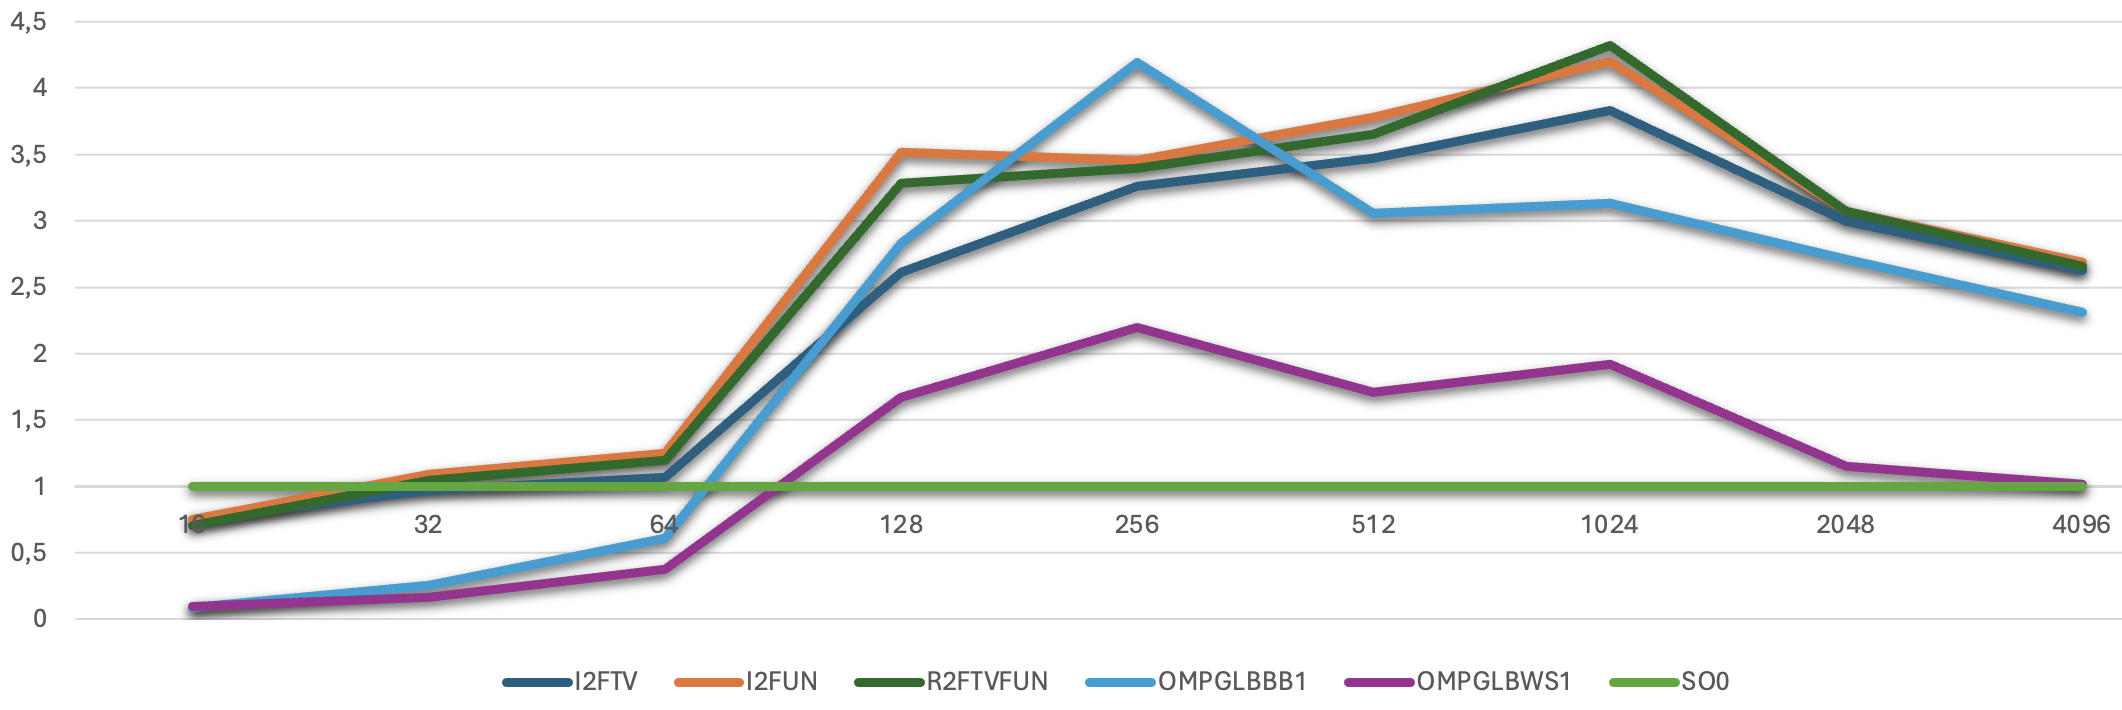
\includegraphics[width=1\columnwidth]{images/Image 1.02.png}
    \caption{Comparison with Sequential (size-speedup)}
    \label{fig:figure1}
\end{figure}
\begin{figure}[!h]
    \centering
    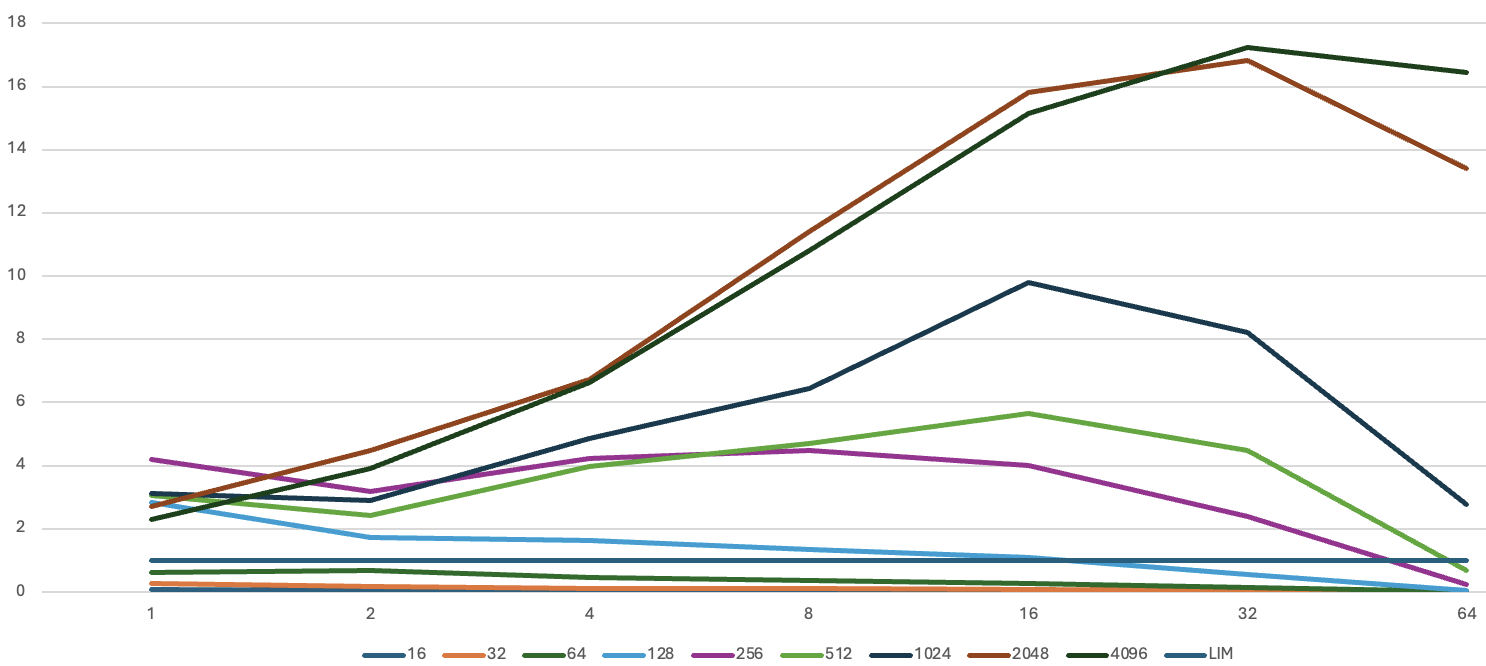
\includegraphics[width=1\columnwidth]{images/Image 1.03.png}
    \caption{Speedup GLB-Block-Based (N° Threads-SpeedUp)}
    \label{fig:figure2}
\end{figure}
\begin{figure}[!h]
    \centering
    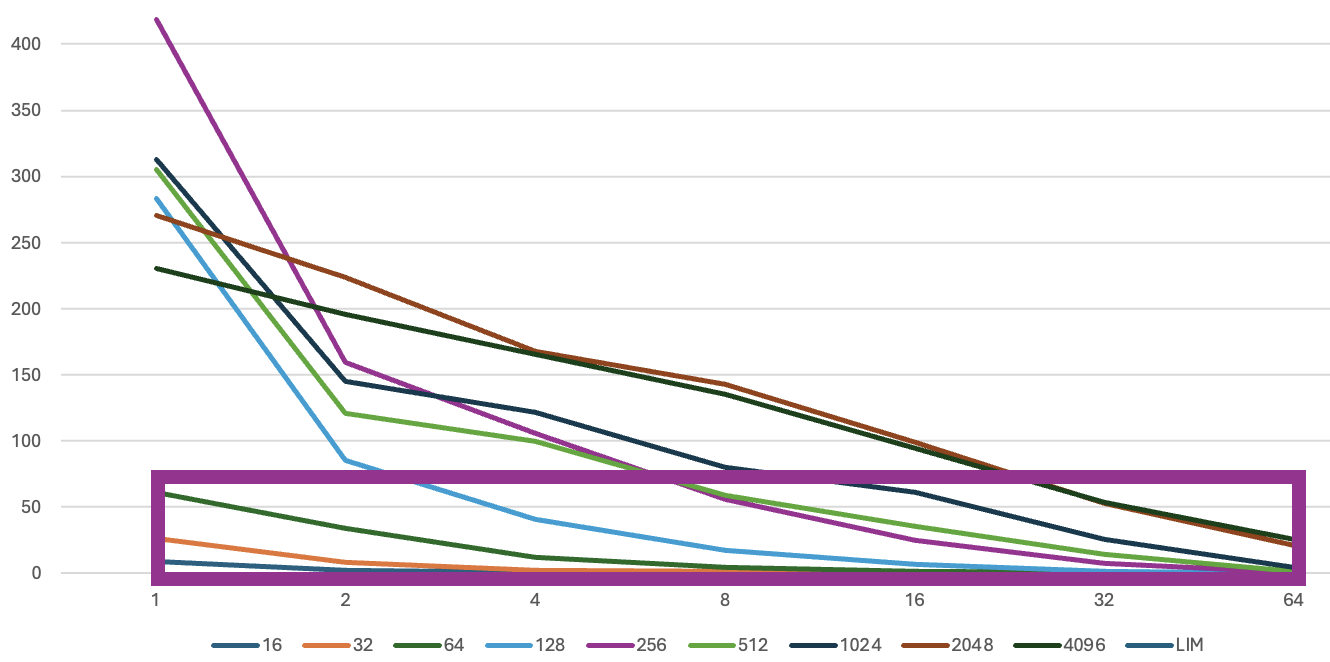
\includegraphics[width=1\columnwidth]{images/Image 1.04.png}
    \caption{Efficiency GLB-Block-Based (N° Threads-Efficiency\%)}
    \label{fig:figure3}
\end{figure}
\if
\fi
\end{document}